\chapter{Compiling and Linking}

\section{How do we compile?}

It's all very well talking about various programming languages and the various syntax that we can use, but when it comes down to creating an executable file that users can work on, we need to understand the process of \emph{compiling} and \emph{linking}. To start with, say we had a file called {\bf simple.c} and we wished to create an executable from this, then we could write in the terminal
\begin{verbatim}
gcc -o output simple.c
\end{verbatim}
which would create an executable name {\bf output}\footnote{Note that if we do not specifiy the output file using the -o flag, then an executable named {\bf a.out} will be created.}. To run this, we can them simply type
\begin{verbatim}
./ouput
\end{verbatim}
Likewise, if we were working with C++ programs, we could type, for example
\begin{verbatim}
g++ -o output simple.cpp
\end{verbatim}
and execute the program using the same command as above. 

But what is going on here? There is some sort of dark magic happening within the computer, and we want to know what it it. In fact, there are three stages:
\begin{enumerate}
\item Compiler stage. Here the source files (eg. in C these would be the files which end in .h and .c) are converted into a lower level language known as assembly language. 
\item Assembler stage. At this point we converted the assembly files into object code which the computer understands directly. These files end in .o
\item Linker stage. The object code is linked to code libraries such as those that allow us to use functions like printf. It is this process which finally produces the executable.
\end{enumerate}

In the previous example we were working with only one file, but in more complex programs the use of several source files will be necessary. This is where the use of a makefile becomes very useful. To understand this, let us first begin with a program consisting of three source files {\bf green.c}, {\bf common..h} and {\bf blue.c}. This could be compiled as 
\begin{verbatim}
gcc -o output green.c blue.c 
\end{verbatim}
What happens here is that the compiler stage produces two assembly files, the assembly stage produces two object files, but at the linking stage \emph{only one executable file is produced}. In actual fact, there are three stages to this process
\begin{enumerate}
\item Create the object file for green.c.
\begin{verbatim}
gcc -c green.c
\end{verbatim}
\item Create the object file for blue.c.
\begin{verbatim}
gcc -c blue.c
\end{verbatim}
\item Link the object files together
\begin{verbatim}
cc green.o blue.o
\end{verbatim}
\end{enumerate}

\section{The makefile}

When we have multiple files in our project, the the makefile becomes a necessity if we want to compile efficiently. To demonstrate a makefile does, it is useful to look at a project made up of multiple files.
\begin{figure}[htbp]
\begin{center}
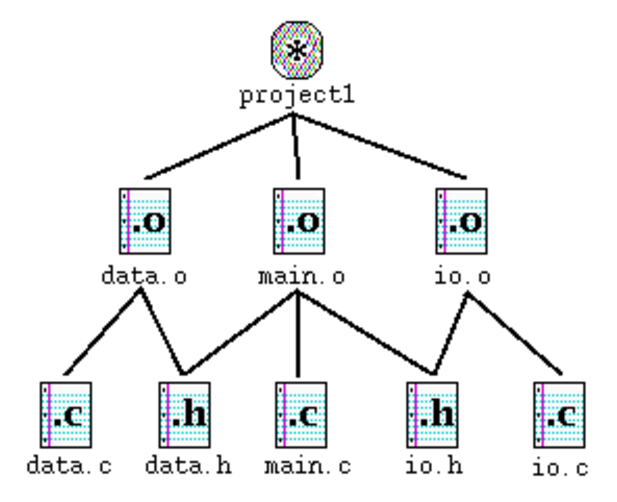
\includegraphics[height=4cm]{figures/depgraph.eps}
\caption{File dependencies in a project}
\label{default}
\end{center}
\end{figure}
\begin{figure}[htbp]
\begin{center}
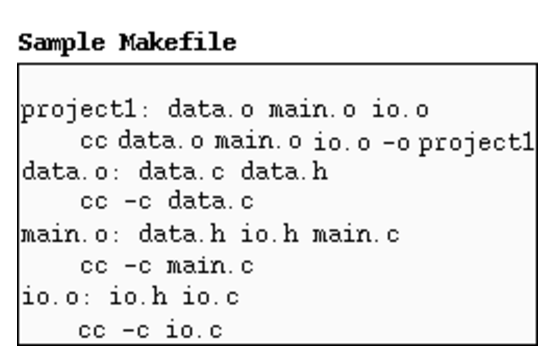
\includegraphics[height=4cm]{figures/makefile.eps}
\caption{The makefile}
\label{default}
\end{center}
\end{figure}
The makefile is made up of the following format:
\begin{verbatim}
target: source file(s)
		       command (note that the tab is required)
\end{verbatim}
and must be named {\bf makefile} or {\bf Makefile} if you wish to use the command ``make''. However it is possible to use a different makefile name by running the following command
\begin{verbatim}
make -f mymakefile
\end{verbatim}

\subsection{My simple makefile test}

I tried my own makefile to see if I could get things working and compile things much faster. I wrote a simple program in C++ contained in one file called 
\begin{verbatim}
mapTester.cpp
\end{verbatim}
I created a makefile as follows:
\begin{verbatim}
CC=g++
CFLAGS=-Wall

mapTester: mapTester.o

clean:
        rm -f mapTester mapTester.o
\end{verbatim}
And voila! When I type 'make' I create a compiled program (if I have changed anything in the source file) and when I type 'make clean' I remove the exectuble and the object file. Brilliant.


%\section{Macros in make}
%We can also use macros to define a set of files. And, since the make command knows that in order to create an object file it must use cc -c on the associated .c file, we can omit these files from the makefile. eg.
%\begin{verbatim}
%OBJECTS = data.o main.o io.o
%project1: $(OBJECTS)
%       cc $(OBJECTS) -o project1
%data.o: data.h
%main.o: data.h io.h
%io.o: io.h
%\end{verbatim}

\section{A more general makefile}

The previous section illustrated a very simple makefile, but in most cases we will end up with a much more complicated scenario where several source files and header files must be compiled and then linked together to produce the desired executable. To do this, Make allows us to make use of certain implicit rules that simplify the creation of a makefile. 

Say we have four source files main.cpp, car.cpp, vehicle.cpp and truck.cpp and three header files car.h, vehicle.h and truck.h.  If we were to compile everything separately, we would find that there would be four object files: main.o, car.o, vehicle.o and truck.o and these are linked together to produce the resulting executable. But Make allows us to compile and link very easily using the following file:
\begin{verbatim}
CC = g++
CFLAGS = -Wall

OBJECTS = main.o vehicle.o car.o truck.o

app : $(OBJECTS)
       $(CC) -o app $(OBJECTS)

main.o : vehicle.h car.h truck.h
vehicle.o : vehicle.h
car.o : car.h
truck.o : truck.h

clean:
       rm app $(OBJECTS)
\end{verbatim}

What might seem strange are the lines which list the dependencies for each of the object files. For example, the line 
\begin{verbatim}
main.o : vehicle.h car.h truck.h
\end{verbatim}
would usually be written as
\begin{verbatim}
main.o : main.cpp vehicle.h car.h truck.h
       $(CC) -c main.cpp 
\end{verbatim}
The reason we can write the latter is because Make has an implicit rule which says that every object file is compiled from a corresponding source file with the same name. And when we write
\begin{verbatim}
main.o : vehicle.h car.h truck.h
\end{verbatim}
it is implicitly assumed that the object is created using
\begin{verbatim}
$(CC) -c 
\end{verbatim}
with the same name as the object file.

\section{CMake}
\label{sec:cmake}

CMake is one of the most important developments for the task of
compiling programs on a variety of platforms. It allows us to worry
less about compiling the code on various machines since it has the
ability to create automatically Xcode project files (for the Mac),
Visual Studio files (for windows) and makefiles (for Linux). The idea
is that all the instructions for compiling and linking are given in a
file called CMakeLists.txt. To demonstrate the process, consider the
following directory structure that we might see in a project:
\begin{verbatim}
src/
include/
main.cpp
CMakeLists.txt
\end{verbatim}
The source files (eg. .cpp files) are kept in /src and header files
are kept in /include (e.g. .h files). The reason for this is to make
life easier if we distribute our code as a library where we must give
our header files alongside the libraries. The main.cpp is the usual
main entry point to our program.

The really interesting part though is the CMakeLists.txt file which
basically replaces the need to manually create a Makefile. In this
project our CMakeLists.txt file might look something like this
\begin{verbatim}
CMAKE_MINIMUM_REQUIRED( VERSION 2.6 )
PROJECT( cmaketest )

# the directory to look for header files
INCLUDE_DIRECTORIES( include )

# using a 'globbing' approach where we find all the .cpp files and make them our source files
FILE( GLOB SOURCES src/*.cpp )
MESSAGE( "SOURCES = " ${SOURCES} )

# define the library path
SET(LIBRARY_OUTPUT_PATH ${cmaketest_BINARY_DIR}/lib)

# create a library
ADD_LIBRARY( mylib ${SOURCES} )

# create an executable
ADD_EXECUTABLE( cmakeTestExec main.cpp )
TARGET_LINK_LIBRARIES( cmakeTestExec mylib )
\end{verbatim}

Let's go through this line by line.

\begin{enumerate}
\item First, we must tell cmake the minimum version of cmake that is
  required. 2.6 seems to be quite common at the moment.
\item Define the project name that will be used in later commands.
\item Tell the compiler where to look for header files when compiling
  (ie. the -I flag).
\item Define a variable called SOURCES which is made up of all the
  source files for our project. In this case we look in the src/
  directory for all files ending in .cpp.
\item Display a message which lists all the source files (as a check
  for the user of cmake).
\item The default library path is the same as the build directory, but
  in this case we have decided to include the libraries in a folder
  called 'lib'. This will be seen in the build directory.
\item We create a library called mylib by compiling the source files.
\item We create an executable from main.cpp.
\item We must link the previously created executable with the library
  we have just created.
\end{enumerate}

\subsection{Using ccmake}
\label{sec:using-ccmake}


What we have done in the previous section is set up the rules that
will allow us to create a ``build'' of the project. That is, we can
create a folder that will contain the executable and library files for
the project after compilation on our machine. Since different
computers have different ``architectures'' we may need to create
several builds for each different type.

Let's assume we are in the directory of the source code which contains
the file main.cpp\footnote{Look in ~/Documents/programming/cmake/cmakeDemo to find these files on my computer}. We can create a build directory here by 
\begin{verbatim}
mkdir build
\end{verbatim}
We can change into this directory with
\begin{verbatim}
cd build/
\end{verbatim}
We can now run ccmake, which is a GUI for cmake as follows:
\begin{verbatim}
ccmake ../
\end{verbatim}
This tell ccmake to look in the directory above for the CMakeLists.txt
file. You will see a table of values which have been automatically
created by CMake. In some cases we might need to change these, like in
the case when we specify the location of a library. But for this
simple project we can simply type
\begin{verbatim}
c
\end{verbatim}
which will show a message of all the source files. We exit this by
typing
\begin{verbatim}
e
\end{verbatim}
We can then generate the makefile by typing
\begin{verbatim}
g
\end{verbatim}
You should now see a makefile in the current directory. This allows us
to compile the code to produce the executable and the library by
simply typing
\begin{verbatim}
make
\end{verbatim}

Essentially, we have greatly simplified the creation of makefiles
which can often be problematic for cross-platform compiling (ie
producing libraries and executables on different machines).

%%% Local Variables: 
%%% mode: latex
%%% TeX-master: "Programming"
%%% End: 
